% Template for PLoS
% Version 3.4 January 2017
\documentclass[10pt,letterpaper]{article}
\usepackage[top=0.85in,left=2.75in,footskip=0.75in]{geometry}

% amsmath and amssymb packages, useful for mathematical formulas and symbols
\usepackage{amsmath,amssymb}

% Use adjustwidth environment to exceed column width (see example table in text)
\usepackage{changepage}

% Use Unicode characters when possible
\usepackage[utf8x]{inputenc}

% textcomp package and marvosym package for additional characters
\usepackage{textcomp,marvosym}

% cite package, to clean up citations in the main text. Do not remove.
% \usepackage{cite}

% Use nameref to cite supporting information files (see Supporting Information section for more info)
\usepackage{nameref,hyperref}

% line numbers
\usepackage[right]{lineno}

% ligatures disabled
\usepackage{microtype}
\DisableLigatures[f]{encoding = *, family = * }

% color can be used to apply background shading to table cells only
\usepackage[table]{xcolor}

% array package and thick rules for tables
\usepackage{array}

% create "+" rule type for thick vertical lines
\newcolumntype{+}{!{\vrule width 2pt}}

% create \thickcline for thick horizontal lines of variable length
\newlength\savedwidth
\newcommand\thickcline[1]{%
  \noalign{\global\savedwidth\arrayrulewidth\global\arrayrulewidth 2pt}%
  \cline{#1}%
  \noalign{\vskip\arrayrulewidth}%
  \noalign{\global\arrayrulewidth\savedwidth}%
}

% \thickhline command for thick horizontal lines that span the table
\newcommand\thickhline{\noalign{\global\savedwidth\arrayrulewidth\global\arrayrulewidth 2pt}%
\hline
\noalign{\global\arrayrulewidth\savedwidth}}


% Remove comment for double spacing
%\usepackage{setspace} 
%\doublespacing

% Text layout
\raggedright
\setlength{\parindent}{0.5cm}
\textwidth 5.25in 
\textheight 8.75in

% Bold the 'Figure #' in the caption and separate it from the title/caption with a period
% Captions will be left justified
\usepackage[aboveskip=1pt,labelfont=bf,labelsep=period,justification=raggedright,singlelinecheck=off]{caption}
\renewcommand{\figurename}{Fig}

% Use the PLoS provided BiBTeX style
% \bibliographystyle{plos2015}

% Remove brackets from numbering in List of References
\makeatletter
\renewcommand{\@biblabel}[1]{\quad#1.}
\makeatother

% Leave date blank
\date{}

% Header and Footer with logo
\usepackage{lastpage,fancyhdr,graphicx}
\usepackage{epstopdf}
\pagestyle{myheadings}
\pagestyle{fancy}
\fancyhf{}
\setlength{\headheight}{27.023pt}
\lhead{\includegraphics[width=2.0in]{PLOS-submission.eps}}
\rfoot{\thepage/\pageref{LastPage}}
\renewcommand{\footrule}{\hrule height 2pt \vspace{2mm}}
\fancyheadoffset[L]{2.25in}
\fancyfootoffset[L]{2.25in}
\lfoot{\sf PLOS}

%% Include all macros below
\newcommand{\lorem}{{\bf LOREM}}
\newcommand{\ipsum}{{\bf IPSUM}}

\usepackage{color}
\usepackage{fancyvrb}
\newcommand{\VerbBar}{|}
\newcommand{\VERB}{\Verb[commandchars=\\\{\}]}
\DefineVerbatimEnvironment{Highlighting}{Verbatim}{commandchars=\\\{\}}
% Add ',fontsize=\small' for more characters per line
\usepackage{framed}
\definecolor{shadecolor}{RGB}{248,248,248}
\newenvironment{Shaded}{\begin{snugshade}}{\end{snugshade}}
\newcommand{\AlertTok}[1]{\textcolor[rgb]{0.94,0.16,0.16}{#1}}
\newcommand{\AnnotationTok}[1]{\textcolor[rgb]{0.56,0.35,0.01}{\textbf{\textit{#1}}}}
\newcommand{\AttributeTok}[1]{\textcolor[rgb]{0.77,0.63,0.00}{#1}}
\newcommand{\BaseNTok}[1]{\textcolor[rgb]{0.00,0.00,0.81}{#1}}
\newcommand{\BuiltInTok}[1]{#1}
\newcommand{\CharTok}[1]{\textcolor[rgb]{0.31,0.60,0.02}{#1}}
\newcommand{\CommentTok}[1]{\textcolor[rgb]{0.56,0.35,0.01}{\textit{#1}}}
\newcommand{\CommentVarTok}[1]{\textcolor[rgb]{0.56,0.35,0.01}{\textbf{\textit{#1}}}}
\newcommand{\ConstantTok}[1]{\textcolor[rgb]{0.00,0.00,0.00}{#1}}
\newcommand{\ControlFlowTok}[1]{\textcolor[rgb]{0.13,0.29,0.53}{\textbf{#1}}}
\newcommand{\DataTypeTok}[1]{\textcolor[rgb]{0.13,0.29,0.53}{#1}}
\newcommand{\DecValTok}[1]{\textcolor[rgb]{0.00,0.00,0.81}{#1}}
\newcommand{\DocumentationTok}[1]{\textcolor[rgb]{0.56,0.35,0.01}{\textbf{\textit{#1}}}}
\newcommand{\ErrorTok}[1]{\textcolor[rgb]{0.64,0.00,0.00}{\textbf{#1}}}
\newcommand{\ExtensionTok}[1]{#1}
\newcommand{\FloatTok}[1]{\textcolor[rgb]{0.00,0.00,0.81}{#1}}
\newcommand{\FunctionTok}[1]{\textcolor[rgb]{0.00,0.00,0.00}{#1}}
\newcommand{\ImportTok}[1]{#1}
\newcommand{\InformationTok}[1]{\textcolor[rgb]{0.56,0.35,0.01}{\textbf{\textit{#1}}}}
\newcommand{\KeywordTok}[1]{\textcolor[rgb]{0.13,0.29,0.53}{\textbf{#1}}}
\newcommand{\NormalTok}[1]{#1}
\newcommand{\OperatorTok}[1]{\textcolor[rgb]{0.81,0.36,0.00}{\textbf{#1}}}
\newcommand{\OtherTok}[1]{\textcolor[rgb]{0.56,0.35,0.01}{#1}}
\newcommand{\PreprocessorTok}[1]{\textcolor[rgb]{0.56,0.35,0.01}{\textit{#1}}}
\newcommand{\RegionMarkerTok}[1]{#1}
\newcommand{\SpecialCharTok}[1]{\textcolor[rgb]{0.00,0.00,0.00}{#1}}
\newcommand{\SpecialStringTok}[1]{\textcolor[rgb]{0.31,0.60,0.02}{#1}}
\newcommand{\StringTok}[1]{\textcolor[rgb]{0.31,0.60,0.02}{#1}}
\newcommand{\VariableTok}[1]{\textcolor[rgb]{0.00,0.00,0.00}{#1}}
\newcommand{\VerbatimStringTok}[1]{\textcolor[rgb]{0.31,0.60,0.02}{#1}}
\newcommand{\WarningTok}[1]{\textcolor[rgb]{0.56,0.35,0.01}{\textbf{\textit{#1}}}}




\usepackage{forarray}
\usepackage{xstring}
\newcommand{\getIndex}[2]{
  \ForEach{,}{\IfEq{#1}{\thislevelitem}{\number\thislevelcount\ExitForEach}{}}{#2}
}

\setcounter{secnumdepth}{0}

\newcommand{\getAff}[1]{
  \getIndex{#1}{Monash University,Genentech}
}

\providecommand{\tightlist}{%
  \setlength{\itemsep}{0pt}\setlength{\parskip}{0pt}}

\begin{document}
\vspace*{0.2in}

% Title must be 250 characters or less.
\begin{flushleft}
{\Large
\textbf\newline{plyranges: a grammar for transforming genomics data} % Please use "sentence case" for title and headings (capitalize only the first word in a title (or heading), the first word in a subtitle (or subheading), and any proper nouns).
}
\newline
\\
Stuart Lee\textsuperscript{\getAff{Monash University}},
Michael Lawrence\textsuperscript{\getAff{Genentech}},
Di Cook\textsuperscript{\getAff{Monash University}}\\
\bigskip
\textbf{\getAff{Monash University}}Department of Econometrics and Business Statistics, Clayton, Victoria,
Australia\\
\textbf{\getAff{Genentech}}Bioinformatics and Computational Biology, Genentech, Inc., South San
Francisco, California, United States of America\\
\bigskip
\end{flushleft}
% Please keep the abstract below 300 words
\section*{Abstract}
The Bioconductor project has created many useful data abstractions for
analysing high-throughput genomics experiments. However, there is a
cognitive load placed on a user in learning a data abstraction and
understanding its appropriate use. Throughout a standard workflow, a
user must navigate and know many of these abstractions to perform an
genomic analysis task, when a single data abstraction, a GRanges object
will suffice. The GRanges class naturally represent genomic intervals
and their associated measurements. By recognising that the GRanges class
follows `tidy' data principles we have created a grammar of genomic data
transformation. The grammar defines verbs for performing actions on and
between genomic interval data. It provides a principled way of
performing common genomic data analysis tasks through a coherent
interface to existing Bioconductor infrastructure, resulting in human
readable analysis workflows. We have implemented this grammar as a
Bioconductor/R package called plyranges.

% Please keep the Author Summary between 150 and 200 words
% Use first person. PLOS ONE authors please skip this step. 
% Author Summary not valid for PLOS ONE submissions.   

\linenumbers

% Use "Eq" instead of "Equation" for equation citations.
\hypertarget{introduction}{%
\section{Introduction}\label{introduction}}

High-throughput genomics promises to unlock new disease therapies, and
strengthen our knowledge of basic biology. To deliver on those promises,
scientists must derive a stream of knowledge from a deluge of data.
Genomic data is challenging in both scale and complexity. Innovations in
sequencing technology often outstrip our capacity to process the output.
Beyond their common association with genomic coordinates, genomic data
are heterogeneous, consisting of raw sequence read alignments, genomic
feature annotations like genes and exons, and summaries like coverage
vectors, ChIP-seq peak calls, variant calls, and per-feature read
counts. Genomic scientists need software tools to wrangle the different
types of data, process the data at scale, test hypotheses, and generate
new ones, all while focusing on the biology, not the computation. For
the tool developer, the challenge is to define ways to model and operate
on the data that align with the mental model of scientists, and to
provide an implementation that scales with their ambition.

Several domain specific languages (DSLs) enable scientists to process
and reason about heterogeneous genomics data by expressing common
operations, such as range manipulation and overlap-based joins, using
the vocabulary of genomics. Their implementations either delegate
computations to a database, or operate over collections of files in
standard formats like BED. An example of the former is the Genome Query
Language (GQL) and its distributed implementation GenAp which use an
SQL-like syntax for fast retrieval of information of unprocessed
sequencing data {[}1{]}; {[}2{]}. Similarly, the Genometric Query
Language (GMQL) implements a relational algebra for combining genomic
datasets {[}3{]}. The command line application BEDtools develops an
extensive algebra for performing arithmetic between two or more sets of
genomic regions {[}4{]}. All of the aforementioned DSLs are designed to
be evaluated either at the command line or embedded in scripts for batch
processing. They exist in a sparse ecosystem, mostly consisting of UNIX
and database tools that lack biological semantics and operate at the
level of files and database tables.

The Bioconductor/R packages \texttt{IRanges} and \texttt{GenomicRanges}
{[}5--7{]} define a DSL for analysing genomics data with R, an
interactive data analysis environment that encourages reproducibility
and provides high-level abstractions for manipulating, modelling and
plotting data, through state of the art methods in statistical
computing. The packages define object-oriented (OO) abstractions for
representing genomic data and enable interoperability by allowing users
and developers to use these abstractions in their own code and packages.
Other genomic DSLs that are embedded in programming languages include
pybedtools and valr {[}8,9{]}, however these packages lack the
interoperability provided by the aforementioned Bioconductor packages
and are not easily extended.

The Bioconductor infrastructure models the genomic data and operations
from the perspective of the power user, one who understands and wants to
take advantage of the subtle differences in data types. This design has
enabled the development of sophisticated tools, as evidenced by the
hundreds of packages depending on the framework. Unfortunately, the
myriad of data structures have overlapping purposes and important but
obscure differences in behavior that often confuse the typical end user.

Recently, there has been a concerted, community effort to standardize R
data structures and workflows around the notion of tidy data {[}10{]}. A
tidy dataset is defined as a tabular data structure that has
observations as rows and columns as variables, and all measurements
pertain to a single observational unit. The tidy data pattern is useful
because it allows us to see how the data relate to the design of an
experiment and the variables measured. The \texttt{dplyr} package
{[}11{]} defines an API that maps notions from the general relational
algebra to operations on tidy data. It expresses each operation as a
cohesive, endomorphic verb. Taken together these features enable a user
to write human readable analysis workflows.

We have created a genomic DSL called \texttt{plyranges} that
reformulates notions from existing genomic algebras and embeds them in R
as a genomic extension of \texttt{dplyr}. By analogy, \texttt{plyranges}
is to the genomic algebra, as \texttt{dplyr} is to the relational
algebra. The \texttt{plyranges} Bioconductor package implements the
language on top of a key subset of Bioconductor data structures and thus
fully integrates with the Bioconductor framework, gaining access to its
scalable data representations and sophisticated statistical methods.

\hypertarget{genomic-relational-algebra}{%
\section{Genomic relational algebra}\label{genomic-relational-algebra}}

\hypertarget{data-model}{%
\subsection{Data model}\label{data-model}}

\begin{figure}
{\centering 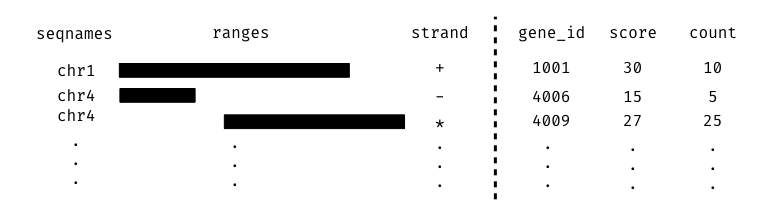
\includegraphics[width=400pt]{diagrams/diagrams-001}}
\caption{An illustration of the GRanges data model for a
sample from an RNA-seq experiment. The core components of the data model
inlcude a seqnames column (representing the chromosome), a ranges column
which consists of start and end coordinates for a genomic region, and a
strand identifier (either positive, negative, or unstranded). Metadata
are included as columns to the right of the dotted line as annotations
(gene\_id) or range level covariates (GC score and count).}
\label{fig:GRanges} 
\end{figure}

The \texttt{plyranges} DSL is built on the core Bioconductor data
structure GRanges, which is capable of representing all types of genomic
data at a semantic level that roughly matches the intuition of most
users. A GRanges is essentially a table, with columns for the
chromosome, start and end coordinates, and the strand, along with an
arbitrary set of additional columns, consisting of measurements or
metadata specific to the data type or experiment (figure
\ref{fig:GRanges}).

\begin{table}[!htbp]
\centering
\begin{tabular}{|l|l|p{4cm}|}
  \hline
  & Verb &  Description \\ 
  \hline
   & \textbf{\emph{summarise()}} & aggregate over column(s) \\ 
   Aggregation & \emph{disjoin\_ranges()} & aggregate column(s) over the union of end coordinates \\
   &  \emph{reduce\_ranges()} & aggregate column(s) by merging overlapping and neighbouring ranges \\
   \hline
   &  \textbf{\emph{mutate()}} & modifies any column \\
   & \textbf{\emph{select()}} & select columns \\
  Arithmetic (Unary) & \textbf{\emph{arrange()}} & sort by columns \\
   & \emph{stretch()} & extend range by fixed amount \\
   &  \emph{shift\_(direction)} & shift coordinates \\
   & \emph{flank\_(direction)} & generate flanking regions \\
   & \emph{\%intersection\% } & row-wise intersection \\
   & \emph{\%union\%} & row-wise union \\
   & \emph{compute\_coverage} & coverage over all ranges \\
  Arithmetic (Binary) &  \emph{\%setdiff\%} & row-wise set difference \\
   & \emph{between()} & row-wise gap range \\
   & \emph{span()} & row-wise spanning range \\
   \hline
    & \emph{join\_overlap\_*()} & merge by overlapping ranges \\
    & \emph{join\_nearest} & merge by nearest neighbour ranges \\
    & \emph{join\_follow} & merge by following ranges \\
    Merging & \emph{join\_precedes} & merge by preceding ranges \\
    & \emph{union\_ranges} & range-wise union \\
    & \emph{intersect\_ranges} & range-wise intersect \\
    & \emph{setdiff\_ranges} & range-wise set difference \\
    & \emph{complement\_ranges} & range-wise union \\
  \hline
   & \textbf{\emph{anchor\_direction()}} & fix coordinates at direction \\
  Modifier & \textbf{\emph{group\_by()}} & partition by column(s)  \\ 
   & \emph{group\_by\_overlaps()} & partition by overlaps \\
   \hline
   & \textbf{\emph{filter()}} & subset rows \\
  Restriction & \emph{filter\_by\_overlaps()} & subset by overlap \\
    & \emph{filter\_by\_non\_overlaps()} & subset by no overlap \\
   \hline
\end{tabular}
\caption{Overview of the \texttt{plyranges} grammar. The core verbs are
briefly described and categorised into one of: aggregation, unary or binary
arithmetic, merging, modifier, or restriction. A verb is given bold text if
its origin is from the \texttt{dplyr} grammar.}\label{tab:grammar}
\end{table}

By definition GRanges follows the tidy data pattern: it is a rectangular
table corresponding to a single biological context. Each row contains a
single observation and each column is a variable about that observation.
Hence, we have designed the \texttt{plyranges} DSL to extend the grammar
and design principles of \texttt{dplyr}: cohesion, consistency,
endomorphism, and fluency. All of these principles are defined and
discussed below in the context of the GRanges class and an overview of
the grammar is provided in table \ref{tab:grammar}. Where applicable we
contrast our design to the existing Bioconductor infrastructure.

\hypertarget{algebraic-operations}{%
\subsection{Algebraic operations}\label{algebraic-operations}}

The \texttt{plyranges} DSL defines an expressive algebra for performing
genomic operations with and between GRanges objects (see table
\ref{tab:grammar}). The grammar includes several classes of operation
that cover most use cases in genomics data analysis. There are operators
for performing arithmetic such as modifying width or performing set
operations, merging such as finding overlaps between GRanges, subsetting
by genomic regions, and aggregating over columns within in a GRanges
object.

GRanges describes the within-sequence coordinates of a range by its
\emph{start}, \emph{end} and \emph{width}. Those three variables are
mutually dependent and partially redundant, so direct manipulation of
them is problematic. For example, changing the \emph{width} column needs
to change either the \emph{start}, \emph{end} or both to preserve
integrity of the object. We introduce the \emph{anchor} modifier to
disambiguate these adjustments. Supported anchor points include the
start, end and midpoint, as well as the 3' and 5' ends for
strand-directed ranges. For example, if we anchor the start, then
setting the width will adjust the end while leaving the start
stationary.

The algebra also defines conveniences for relative coordinate
adjustments: \emph{shift} (unanchored adjustment to both start and end)
and \emph{stretch} (anchored adjustment of width). We can perform any
relative adjustment by some combination of those two operations. The
\emph{stretch} operation requires an anchor and assumes the midpoint by
default. Since \emph{shift} is unanchored, the user specifies a suffix
for indicating the direction: left/right or, for stranded features,
upstream/downstream. For example, \emph{shift\_right} shifts a range to
the right.

The \emph{flank} operation generates new ranges that are adjacent to
existing ones. This is useful, for example, when generating upstream
promoter regions for genes. Analogous to \emph{shift}, a suffix
indicates the side of the input range to flank.

As with other genomic grammars, we define set operations that treat
ranges as sets of integers, including \emph{intersect}, \emph{union},
\emph{difference}, and \emph{complement}. There are two sets of these:
parallel and merging. The parallel operations map to infix operators,
which we surround with \emph{\%} symbols in accordance with R syntax
rules. For example, the parallel intersection (\emph{x \%intersect\% y})
finds the intersecting range between \emph{xi} and \emph{yi} for
\emph{i} in \emph{1\ldots{}n}, where \emph{n} is the length of both
\emph{x} and \emph{y}. In constrast, the merging intersection
(\emph{intersect\_ranges(x, y)}) returns a new set of disjoint ranges
representing whereever there was overlap between a range in \emph{x} and
a range in \emph{y}. We use the infix syntax for the parallel
operations, since it is the conventional syntax for parallel, binary
operations in R. Finding the parallel union will fail when two ranges
have a gap, so we introduce a \emph{span} operator that takes the union
while filling any gap. The \emph{complement} operation is unique in that
it is unary. It finds the regions not covered by any of the ranges in a
single set. Closely related is the \emph{between} parallel operation,
which finds the gap separating \emph{xi} and \emph{yi}. The binary
operations are callable from within the arithmetic, restriction and
aggregation expressions.

Our algebra recasts finding overlaps or nearest neighbours between two
genomic regions as variants of the relational join operator. A join acts
on two GRanges objects, a query and a subject. The join operator is
relational in the sense that metadata from the query and subject ranges
is retained in the joined range. All join operators in the
\texttt{plyranges} DSL generate a set of hits based on overlap or
proximity of ranges and use those hits to merge the two datasets in
different ways. There are four supported matching algorithms:
\emph{overlap}, \emph{nearest}, \emph{precede}, and \emph{follow}. We
can further restrict the matching by whether the query is completely
\emph{within} the subject, and adding the \emph{directed} suffix ensures
that matching ranges have the same direction (strand).

For merging based on the hits, we have three modes: \emph{inner},
\emph{intersect} and \emph{left}. The \emph{inner} overlap join is
similar to the conventional inner join in that there is a row in the
result for every match. A major difference is that the matching is not
by identity, so we have to choose one of the ranges from each pair. We
always choose the left range. The \emph{intersect} join uses the
intersection instead of the left range. Finally, the overlap \emph{left}
join is akin to left outer join in Cobb's relational algebra: it
performs an overlap inner join but also returns all query ranges that
are not hit by the subject.

\begin{figure}

{\centering 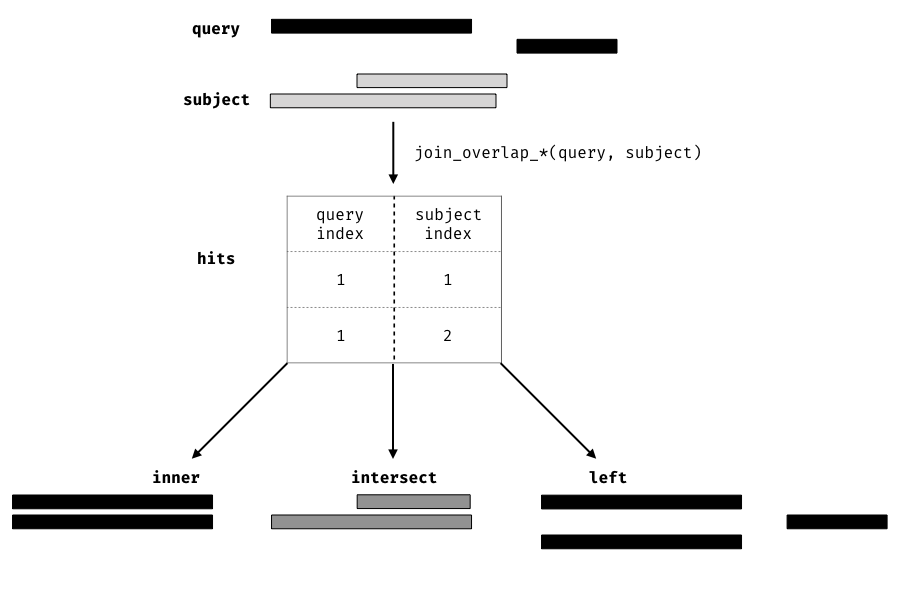
\includegraphics[width=400pt]{diagrams/diagrams-002} 

}

\caption{Illustration of the three overlap join operators. Each join takes query and subject range as input (black and light gray rectangles, respectively). An index for the join is computed, returning a Hits object, which contains the indices of where the subject overlaps the query range. This index is used to expand the query ranges by where it was 'hit' by the subject ranges. The join semantics alter what is returned: for an *inner* join the query range is returned for each match, for an intersect *join* the intersection is taken between overlapping ranges, and for a *left* join all query ranges are returned even if the subject range does not overlap them. This principle is gnerally applied through the `plyranges` DSL for both overlaps and nearest neighbour operations.}\label{fig:olaps-fig}
\end{figure}

Since the GRanges object is a tabular data structure our grammar
includes operators to filter, sort and aggregate by columns in a
GRanges. These operations can be performed over partitions within
GRanges object using the \emph{group\_by} modifier. Together with our
algebra for arithmetic and merging, these operations enable flexible and
reproducible analysis using the desgin principles of the \texttt{dplyr}
grammar.

\hypertarget{cohesion}{%
\subsection{Cohesion}\label{cohesion}}

A function is cohesive if it performs a singular task and does not
produce any side-effects. In the \texttt{plyranges} DSL our algebra for
performing genomic arithmetic is a key example of cohesion. We define
anchoring operators that decorate a GRanges object with an `anchor' and
modify the semantics of performing genomic arithmetic. The anchoring
operators amount to fixing a GRanges object by its start, center, or end
coordinates (or fixing these coordinates by strand). This enables any
arithmetic function that performs a coordinate transformation to remain
cohesive: that is they always perform the same operation regardless of
whether a GRanges object is anchored or not. The only difference is the
result of performing the arithmetic changes when contextual information
is added to the GRanges object.

Another example of our algebra altering object semantics, while
maintaining cohesion is through the `group\_by' operator. Like
anchoring, this operator decorates a GRanges object with a column name
(or names) that defines a partitioning of the GRanges by the unique
values in the column(s). Functions defined in the \texttt{plyranges} DSL
that perform restriction, aggregation, or column modification still
perform those singular tasks, however grouping changes how those tasks
are performed.

\hypertarget{consistency}{%
\subsection{Consistency}\label{consistency}}

A core design principle of the \texttt{plyranges} DSL is interface
consistency: a user should not be surprised by the input or output of
\texttt{plyranges} code. A key example of consistency is how
\texttt{plyranges} handles strand information. Every function that
computes with strand information indicates its intentions by including
suffixes such as `directed', `upstream' or `downstream' in its name,
otherwise strand is ignored. This strongly differs from the Bioconductor
packages, which produces surprising output by assuming the user is
always interested in using strand in the majority of circumstances
(unless a user is computing coverage or finding flanking ranges).

Our use of suffixes in function names, also highlights are core tenet of
the \texttt{plyranges} design: avoid complex generic functions with many
arguments and instead use cohesive functions with a minimal number of
arguments. As an example, we have written a consistent framework for
reading and writing files from and to common genomic data formats as
GRanges, using the \texttt{rtracklayer} package as a back-end {[}12{]}.
We have replaced that packages generic functions for importing files
with a family of reader functions that all take the exact same
arguments.

\hypertarget{endomorphism}{%
\subsection{Endomorphism}\label{endomorphism}}

Most function calls in \texttt{plyranges} are endomorphisms: when the
input is GRanges object the output will also be a GRanges object. The
use of endomorphism in the \texttt{plyranges} DSL enables a user to
predict the structure of the output of their computations and does not
require them to learn any additional classes beyond GRanges and
DataFrames.

As an example, in \texttt{plyranges} when we compute coverage over a
GRanges object, the result of the operation is an expanded GRanges
object with a score column, corresponding the estimated coverage over a
genomic region. Hence, the resulting coverage score can easily be
composed with other expressions in our algebra. This pattern strongly
deviates from the design of the OO interface in \texttt{GenomicRanges},
which in the case of computing coverage would return an RleList, an
object that has many new methods and that is potentially unfamiliar to a
new user. While, these low-level classes enable efficient computing, the
increase complexity, and as a consequence are abstracted away in the
\texttt{plyranges} DSL.

\hypertarget{fluency}{%
\subsection{Fluency}\label{fluency}}

As a consequence of the design principles defined above every function
in \texttt{plyranges} performs a single action on GRanges objects. The
\texttt{plyranges} DSL implements the core verbs from the \texttt{dplyr}
package and implements a genomic relational algebra for transforming
GRanges objects (table x, y). Each verb preserves the semantics of
GRanges object and works with derivatives of the GRanges class. Both of
these aspects reduce the cognitive load on a new user since most
manipulations can be performed with a vocabulary of several verbs,
rather than having to memorise function names that are nouns.

This approach strongly contrasts the \texttt{GenomicRanges/IRanges} OO
interface, which emphasises the use of setter and getter methods. In
that interface, core components and metadata are updated via replacement
methods (requiring knowledge of the class components), while our
interface requires only a single call to \texttt{mutate()} to perform
the modification.

Workflows can be composed by chaining verbs together into `sentences'
via the forward pipe operator,\texttt{\%\textgreater{}\%} (exported from
the R package \texttt{magrittr} {[}13{]}), which can be read as the word
`then'. Overall, this allows users to write human readable code because
workflows describe what the code is doing rather than how its doing it.

\hypertarget{opportunities}{%
\subsection{Opportunities}\label{opportunities}}

A caveat to constructing a compatible interface with \texttt{dplyr} is
that \texttt{plyranges} makes extensive use of non-standard evaluation
in R (achieved via the \texttt{rlang} package {[}14{]}). Simply, this
means that computations are performed and evaluated in the context of
the GRanges objects; emphasising the interactive nature of our API.
Consequently, when programming with \texttt{plyranges} a user needs to
be aware of how non-standard evaluation in R works and how to adapt
their code accordingly. However, with the rise of R packages like
\texttt{rlang} this process is becoming less difficult.

While GRanges are an intuitive representation for data measured on
genomic regions, more flexible data structures are required to represent
data from multiple sample experiments. The Bionconductor class
SummarizedExperiment is the canonical data structure for representing
data for combining multiomic measurements from multiple samples. The
grammar and design of the \texttt{plryanges} DSL can be naturally
extended to the SummarizedExperiment.

\hypertarget{results}{%
\section{Results}\label{results}}

Here we provide illustrative examples by using the \texttt{plyranges}
DSL to show how our grammar could be integrated into genomic data
workflows. We also highlight how interoperability with existing
Bioconductor infrastructure, enables easy access to public datasets and
methods for analysis and visualisation.

\hypertarget{peak-finding}{%
\subsection{Peak Finding}\label{peak-finding}}

The Bioconductor package \texttt{AnnotationHub} {[}15{]} can be used to
search for BigWig files from ChIP-Seq experiments from the Human
Epigenome Roadmap project {[}16{]}. Here we focus on assays for primary
T CD8+ memory cells from peripheral blood. Using \texttt{plyranges} we
will read the BigWig file corresponding to the H3 lysine 27
trimethylation (H3K27Me3) methylation mark over chromosome 10.

First, we gather the BigWig file and extract its annotation information
and filter it to chromosome 10.

\begin{Shaded}
\begin{Highlighting}[]
\KeywordTok{library}\NormalTok{(plyranges)}
\NormalTok{chr10_ranges <-}\StringTok{ }\NormalTok{bw_file }\OperatorTok\StringTok{ }
\StringTok{  }\KeywordTok{get_genome_info}\NormalTok{() }\OperatorTok
\StringTok{  }\KeywordTok{filter}\NormalTok{(seqnames }\OperatorTok{==}\StringTok{ "chr10"}\NormalTok{)}
\end{Highlighting}
\end{Shaded}

Then we read the BigWig file only extracting scores if they overlap
chromosome 10. The annotation information from the file is automatically
included (in this case the hg19 genome build).

\begin{Shaded}
\begin{Highlighting}[]
\NormalTok{chr10_scores <-}\StringTok{ }\NormalTok{bw_file }\OperatorTok
\StringTok{  }\KeywordTok{read_bigwig}\NormalTok{(}\DataTypeTok{overlap_ranges =}\NormalTok{ chr10_ranges) }\OperatorTok
\StringTok{  }\KeywordTok{set_genome_info}\NormalTok{(}\DataTypeTok{genome =} \StringTok{"hg19"}\NormalTok{)}
\end{Highlighting}
\end{Shaded}

The \texttt{reduce\_ranges()} operation is used to find coverage peaks
across chromosome 10. We can manually set a threshold to restrict
genomic regions to have a coverage score of greater than 8, and then
merge nearby regions. The maximum coverage is computed over all the
coverage scores in the regions that were reduced.

\begin{Shaded}
\begin{Highlighting}[]
\NormalTok{all_peaks <-}\StringTok{ }\NormalTok{chr10_scores }\OperatorTok\StringTok{ }
\StringTok{  }\KeywordTok{filter}\NormalTok{(score }\OperatorTok{>}\StringTok{ }\DecValTok{8}\NormalTok{) }\OperatorTok\StringTok{ }
\StringTok{  }\KeywordTok{reduce_ranges}\NormalTok{(}\DataTypeTok{score =} \KeywordTok{max}\NormalTok{(score))}
\end{Highlighting}
\end{Shaded}

Returning to the GRanges object containing normalised coverage scores,
we filter to find the coordinates of the peak containing the maximum
coverage score. We can then find a 5000 nt region centered around the
maximum position by anchoring and modifying the the width.

\begin{Shaded}
\begin{Highlighting}[]
\NormalTok{chr10_max_score_region <-}\StringTok{ }\NormalTok{chr10_scores }\OperatorTok
\StringTok{  }\KeywordTok{filter}\NormalTok{(score }\OperatorTok{==}\StringTok{ }\KeywordTok{max}\NormalTok{(score)) }\OperatorTok\StringTok{ }
\StringTok{  }\KeywordTok{anchor_center}\NormalTok{() }\OperatorTok
\StringTok{  }\KeywordTok{mutate}\NormalTok{(}\DataTypeTok{width =} \DecValTok{5000}\NormalTok{)}
\end{Highlighting}
\end{Shaded}

Finally, the overlap inner join is used to restrict the chromosome 10
normalised coverage scores that are within the 5000nt region that
contain the max peak on chromosome 10 (figure \ref{fig:peak-viz}).

\begin{Shaded}
\begin{Highlighting}[]
\NormalTok{peak_region <-}\StringTok{ }\NormalTok{chr10_scores }\OperatorTok
\StringTok{  }\KeywordTok{join_overlap_inner}\NormalTok{(chr10_max_score_region)}
\end{Highlighting}
\end{Shaded}

\begin{figure}

{\centering 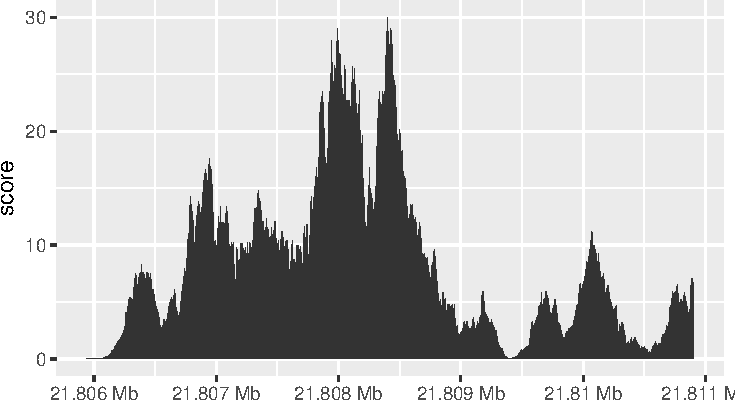
\includegraphics{paper_files/figure-latex/peak-viz-1} 

}

\caption{Visualisation of normalised coverage scores accross a 5000nt region of chromosome 10 from H3K27Me3 ChIP-Seq assay from the Human Epigenome Roadmap project.}\label{fig:peak-viz}
\end{figure}

\hypertarget{computing-windowed-statistics}{%
\subsection{Computing Windowed
Statistics}\label{computing-windowed-statistics}}

Another common operation in genomics data analysis is to compute data
summaries over genomic windows. In \texttt{plyranges} this can be
achieved via the \texttt{group\_by\_overlaps} operator. Continuing with
the data from the Human Epigenome Roadmap Consortium data, we can count
the number of reads that fall into a fixed bins of size 10000bp over a
BAM file of H3K27Me3 methylation marks from the H1 cell line. We extract
reads that have a mapping quality score greater than 20:

\begin{Shaded}
\begin{Highlighting}[]
\NormalTok{alignments <-}\StringTok{ }\KeywordTok{read_bam}\NormalTok{(h1_bam) }\OperatorTok
\StringTok{  }\KeywordTok{filter}\NormalTok{(mapq }\OperatorTok{>}\StringTok{ }\DecValTok{20}\NormalTok{) }
\end{Highlighting}
\end{Shaded}

Note that the BAM file is only read into memory once we perform an
operation on it. Because of interoperability over Bioconductor, we can
generate genomic bins using the \texttt{tile} function from
\texttt{GenomicRanges}:

\begin{Shaded}
\begin{Highlighting}[]
\NormalTok{bins <-}\StringTok{ }\KeywordTok{tile}\NormalTok{(h1_bam, }\DataTypeTok{width =} \DecValTok{10000}\NormalTok{)}
\end{Highlighting}
\end{Shaded}

Finally, we can use \texttt{group\_by\_overlaps} with \texttt{summarise}
to compute the total number of reads within each window.

\begin{Shaded}
\begin{Highlighting}[]
\NormalTok{h1_bam_read_summary <-}\StringTok{ }\NormalTok{h1_bam }\OperatorTok
\StringTok{  }\KeywordTok{group_by_overlaps}\NormalTok{(bins) }\OperatorTok
\StringTok{  }\KeywordTok{summarise}\NormalTok{(}\DataTypeTok{n_reads =} \KeywordTok{n}\NormalTok{())}
\end{Highlighting}
\end{Shaded}

\hypertarget{quality-control-metrics}{%
\subsection{Quality Control Metrics}\label{quality-control-metrics}}

We have created a GRanges object from genotyping performed on the H1
cell line, consisting of approximately two million single nucleotide
polymorphisms (SNP) and short insertion/deletions (indel). The GRanges
object consists of 7 columns, relating to the alleles of a SNP or indel,
the B-allele frequency, log relative intensity of the probes, GC content
score over a probe, and the name of the probe. We can use this
information to compute the transition-transversion ratio, a quality
control metric, within each chromosome in GRanges object.

First we filter out any insertion or deletion alleles and the SNPs
present on the mitochondria then create a logical vector corresponding
to whether there is a transition event.

\begin{Shaded}
\begin{Highlighting}[]
\NormalTok{h1_snp_array <-}\StringTok{ }\NormalTok{h1_snp_array }\OperatorTok
\StringTok{  }\KeywordTok{filter}\NormalTok{(}\OperatorTok{!}\NormalTok{(ref }\OperatorTok\StringTok{ }\KeywordTok{c}\NormalTok{(}\StringTok{"I"}\NormalTok{, }\StringTok{"D"}\NormalTok{)), seqnames }\OperatorTok{!=}\StringTok{ "M"}\NormalTok{) }\OperatorTok
\StringTok{  }\KeywordTok{mutate}\NormalTok{(}\DataTypeTok{transition =}\NormalTok{ (ref }\OperatorTok\StringTok{ }\KeywordTok{c}\NormalTok{(}\StringTok{"A"}\NormalTok{, }\StringTok{"G"}\NormalTok{) }\OperatorTok{&}\StringTok{ }\NormalTok{alt }\OperatorTok\StringTok{ }\KeywordTok{c}\NormalTok{(}\StringTok{"G"}\NormalTok{,}\StringTok{"A"}\NormalTok{)) }\OperatorTok{|}
\StringTok{                      }\NormalTok{(ref }\OperatorTok\StringTok{ }\KeywordTok{c}\NormalTok{(}\StringTok{"C"}\NormalTok{,}\StringTok{"T"}\NormalTok{) }\OperatorTok{&}\StringTok{ }\NormalTok{alt }\OperatorTok\StringTok{ }\KeywordTok{c}\NormalTok{(}\StringTok{"T"}\NormalTok{, }\StringTok{"C"}\NormalTok{)))}
\end{Highlighting}
\end{Shaded}

We can then compute the transition-transversion ratio using the
\texttt{group\_by} and \texttt{summarise} pattern, it is computed as the
total number of transition SNPs divided by the total number of
transversion SNPs within each chromosome (figure \ref{fig:titv-viz}).

\begin{Shaded}
\begin{Highlighting}[]
\NormalTok{ti_tv_results <-}\StringTok{ }\NormalTok{h1_snp_array }\OperatorTok\StringTok{ }
\StringTok{  }\KeywordTok{group_by}\NormalTok{(seqnames) }\OperatorTok
\StringTok{  }\KeywordTok{summarise}\NormalTok{(}\DataTypeTok{n_snps =} \KeywordTok{n}\NormalTok{(),}
            \DataTypeTok{ti_tv =} \KeywordTok{sum}\NormalTok{(transition) }\OperatorTok{/}\StringTok{ }\KeywordTok{sum}\NormalTok{(}\OperatorTok{!}\NormalTok{transition)) }
\end{Highlighting}
\end{Shaded}

\begin{figure}

{\centering 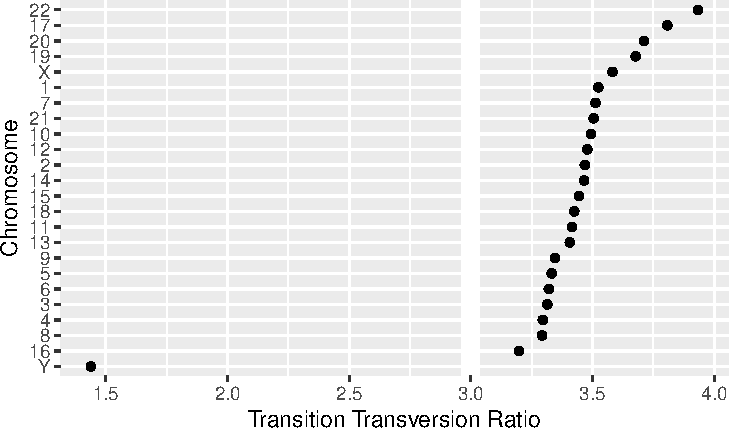
\includegraphics{paper_files/figure-latex/titv-viz-1} 

}

\caption{Dot plot of chromosomes ordered by estimated transition-transversion ratio. A white reference line is drawn at the expected ratio for a human exome.}\label{fig:titv-viz}
\end{figure}

\hypertarget{availablilty-and-future-work}{%
\section{Availablilty and Future
Work}\label{availablilty-and-future-work}}

The \texttt{plyranges} package is available on the Bioconductor project
website \url{https://bioconductor.org} or can be accessed via Github
\url{https://github.com/sa-lee/plyranges}. We aim to continue developing
the \texttt{plyranges} package and extend it for use with more complex
data structures such as the SummarizedExperiment class, which can be
used for analysing transcriptomic and variant data. As the
\texttt{plyranges} interface encourages tidy data practices it
integrates well with the principles of the grammar of graphics, we aim
to use it to prepare data for the visualisation of multimodal biological
datasets.

\hypertarget{acknowledgements}{%
\section{Acknowledgements}\label{acknowledgements}}

We would like to thank Dr Matthew Ritchie at the Walter and Eliza Hall
Institute and Dr Paul Harrison for their feedback on earlier drafts of
this work. We would also like to thank Lori Shepherd and Hèrve Pages for
the code review they performed. This report was written with
\texttt{knitr} {[}17{]} and the figures were made with \texttt{ggbio}
{[}18{]}. All code required to reproduce this article is available at
https://github.com/sa-lee/plyranges-paper.

\hypertarget{references}{%
\section*{References}\label{references}}
\addcontentsline{toc}{section}{References}

\hypertarget{refs}{}
\leavevmode\hypertarget{ref-Kozanitis2014-va}{}%
1. Kozanitis C, Heiberg A, Varghese G, Bafna V. Using genome query
language to uncover genetic variation. Bioinformatics. 2014;30: 1--8.
doi:\href{https://doi.org/10.1093/bioinformatics/btt250}{10.1093/bioinformatics/btt250}

\leavevmode\hypertarget{ref-Kozanitis2016-bm}{}%
2. Kozanitis C, Patterson DA. GenAp: A distributed SQL interface for
genomic data. BMC Bioinformatics. 2016;17: 63.
doi:\href{https://doi.org/10.1186/s12859-016-0904-1}{10.1186/s12859-016-0904-1}

\leavevmode\hypertarget{ref-Kaitoua2017-pw}{}%
3. Kaitoua A, Pinoli P, Bertoni M, Ceri S. Framework for supporting
genomic operations. IEEE Trans Comput. 2017;66: 443--457.
doi:\href{https://doi.org/10.1109/TC.2016.2603980}{10.1109/TC.2016.2603980}

\leavevmode\hypertarget{ref-Quinlan2010-gc}{}%
4. Quinlan AR, Hall IM. BEDTools: A flexible suite of utilities for
comparing genomic features. Bioinformatics. 2010;26: 841--842.
doi:\href{https://doi.org/10.1093/bioinformatics/btq033}{10.1093/bioinformatics/btq033}

\leavevmode\hypertarget{ref-r-core}{}%
5. R Core Team. R: A language and environment for statistical computing
{[}Internet{]}. Vienna, Austria: R Foundation for Statistical Computing;
2018. Available: \url{https://www.R-project.org/}

\leavevmode\hypertarget{ref-Lawrence2013-wg}{}%
6. Lawrence M, Huber W, Pagès H, Aboyoun P, Carlson M, Gentleman R, et
al. Software for computing and annotating genomic ranges. PLoS Comput
Biol. 2013;9.
doi:\href{https://doi.org/10.1371/journal.pcbi.1003118}{10.1371/journal.pcbi.1003118}

\leavevmode\hypertarget{ref-Huber2015-ei}{}%
7. Huber W, Carey VJ, Gentleman R, Anders S, Carlson M, Carvalho BS, et
al. Orchestrating high-throughput genomic analysis with bioconductor.
Nat Methods. Springer Nature; 2015;12: 115--121.
doi:\href{https://doi.org/10.1038/nmeth.3252}{10.1038/nmeth.3252}

\leavevmode\hypertarget{ref-Dale2011-js}{}%
8. Dale RK, Pedersen BS, Quinlan AR. Pybedtools: A flexible python
library for manipulating genomic datasets and annotations.
Bioinformatics. 2011;27: 3423--3424.
doi:\href{https://doi.org/10.1093/bioinformatics/btr539}{10.1093/bioinformatics/btr539}

\leavevmode\hypertarget{ref-Kent2017}{}%
9. Riemondy KA, Sheridan RM, Gillen A, Yu Y, Bennett CG, Hesselberth JR.
Valr: Reproducible genome interval arithmetic in r. F1000Research. 2017;
doi:\href{https://doi.org/10.12688/f1000research.11997.1}{10.12688/f1000research.11997.1}

\leavevmode\hypertarget{ref-Wickham2014-jc}{}%
10. Wickham H. Tidy data. Journal of Statistical Software, Articles.
2014;59: 1--23.
doi:\href{https://doi.org/10.18637/jss.v059.i10}{10.18637/jss.v059.i10}

\leavevmode\hypertarget{ref-Wickham2017-dplyr}{}%
11. Wickham H, Francois R, Henry L, Müller K. Dplyr: A grammar of data
manipulation {[}Internet{]}. 2017. Available:
\url{https://CRAN.R-project.org/package=dplyr}

\leavevmode\hypertarget{ref-Lawrence2009-nt}{}%
12. Lawrence M, Gentleman R, Carey V. Rtracklayer: An R package for
interfacing with genome browsers. Bioinformatics. 2009;25: 1841--1842.
doi:\href{https://doi.org/10.1093/bioinformatics/btp328}{10.1093/bioinformatics/btp328}

\leavevmode\hypertarget{ref-R-magrittr}{}%
13. Bache SM, Wickham H. Magrittr: A forward-pipe operator for r
{[}Internet{]}. 2014. Available:
\url{https://CRAN.R-project.org/package=magrittr}

\leavevmode\hypertarget{ref-R-rlang}{}%
14. Henry L, Wickham H. Rlang: Functions for base types and core r and
'tidyverse' features {[}Internet{]}. 2017. Available:
\url{http://rlang.tidyverse.org}

\leavevmode\hypertarget{ref-R-ahub}{}%
15. Morgan M. AnnotationHub: Client to access annotationhub resources.
2017.

\leavevmode\hypertarget{ref-Roadmap_Epigenomics_Consortium2015-pr}{}%
16. Roadmap Epigenomics Consortium, Kundaje A, Meuleman W, Ernst J,
Bilenky M, Yen A, et al. Integrative analysis of 111 reference human
epigenomes. Nature. 2015;518: 317--330.
doi:\href{https://doi.org/10.1038/nature14248}{10.1038/nature14248}

\leavevmode\hypertarget{ref-R-knitr}{}%
17. Xie Y. Dynamic documents with R and knitr {[}Internet{]}. 2nd ed.
Boca Raton, Florida: Chapman; Hall/CRC; 2015. Available:
\url{https://yihui.name/knitr/}

\leavevmode\hypertarget{ref-R-ggbio}{}%
18. Yin T, Cook D, Lawrence M. Ggbio: An r package for extending the
grammar of graphics for genomic data. Genome Biology. BioMed Central
Ltd; 2012;13: R77.

\nolinenumbers


\end{document}

